\chapter{Implementação}

O conjunto de sistemas embarcados propostos são integrados em um Controlador Semafórico, dispondo um meio de monitorar, controlar e gerenciar os vários aspectos envolvidos no ambiente urbano, em relação ao trânsito. O controlador semafórico é uma solução que envolve diferentes equipamentos, com objetivos específicos cada, que interligados apresentam um meio de ordenar o fluxo veicular e de pedestres em seu entorno.

Com a utilização de microcontroladores, o planejamento de circuitos eletrônicos e a programação de \textit{firmwares} dedicados, o controlador semafórico é responsável por realizar o acendimento e monitoramento da sinalização semafórica, sendo suas funções mais relevantes para tal solução: acendimento de grupos focais (lâmpadas de semáforos) veiculares, acendimento de grupos focais para pedestres, detecção de demanda de travessia de pedestres, sinalização de tempo restante de passagem de veículos (\textit{display} acoplado aos grupos focais, exibindo um contador regressivo).

Cada sistema, individualmente, possui um propósito específico, e foi planejado de modo otimizado, para apresentar confiabilidade, fácil funcionamento e custo reduzido.


\section{Placa de CPU}

A placa de CPU é responsável por determinar o funcionamento das demais placas do controlador. Por meio de um canal de comunicação com as placas de controle de acendimento semafórico e de detecção de demanda de atuadores externos, a CPU envia comandos que regem o comportamento do sistema como um todo.

O controlador pode ser acessado, por meio de uma central, com a qual a placa de CPU se comunica, permitindo assim a modificação de parâmetros do sistema, em tempo real. Desse modo, o controlador semafórico funciona de maneira automatizada, podendo ter suas configurações modificadas por meio de acesso remoto.

É possível, ainda, que o controlador tenha um modo de funcionamento adaptativo, em que os tempos de acendimento não sejam fixos. Nesse modo, o controlador deve realizar leituras em detectores, instalados nas vias, e processar essas informações para definir como o semáforo irá se comportar.
O processamento dos dados pode ser realizado diretamente pela CPU do controlador, ou pode ser realizado externamente, por um servidor que possui comunicação com o sistema.

\section{Placa de controle de acendimento semafórico}

A placa de controle de acendimento semafórico tem como função assegurar o funcionamento correto do semáforo, tanto veicular quanto de pedestres, sendo responsável pelo acendimento e monitoramento dos focos, assegurando a sequência correta de cores do semáforo (Verde > Amarelo > Vermelho)\cite{CET}.
%[http://meusite.mackenzie.br/professor_cucci/ManualSemaforos2014.pdf]. 

O microcontrolador utilizado na placa é um PIC16F77, que possui 40 pinos e capacidade de processamento de 8 \textit{bits}. Um cristal é utilizado, para gerar uma velocidade de \textit{clock} de 20 MHz, e cada instrução é realizada a cada 200 ns (4 ciclos do \textit{clock}). Esse dispositivo é utilizado para chavear a tensão da rede elétrica e monitorar o acendimento semafórico, e enviar as informações para a central do controlador semafórico.

O \textit{firmware} da placa foi escrito especificamente para o dispositivo utilizado realizar as funções desejadas. A placa aguarda os comandos vindos da \ac{CPU} do controlador semafórico para executar o acendimento dos focos. Os comandos são recebidos pela porta serial (\ac{USART}) do PIC16F77, através de comunicação assíncrona.

O PIC16F77 possui um \ac{ADC} com precisão de 8 \textit{bits}, que é utilizado, no projeto, para realizar a leitura do valor da tensão da carga, que é o foco, quando aceso. O sinal passa por um transformador abaixador e uma ponte retificadora, para ser lido pelo pino do PIC, que resulta em um valor de leitura proporcional à potência da carga utilizada. Esse circuito permite ao sistema ter capacidade de monitorar diversos estados das lâmpadas utilizadas no semáforo, sendo eles subtensão, funcionamento esperado, sobretensão e queima.

Outra função da placa é o monitoramento de acendimento dos focos, em que o PIC realiza a leitura de cada foco (verde, amarelo, vermelho) de uma fase e armazena os valores lidos. A leitura é realizada no pino de saída de um optoacoplador, o qual é ativado pela presença de fase e neutro (rede elétrica) na sua entrada. A placa possui um circuito separado para cada foco monitorado, cada um ocupando um pino diferente de \ac{I/O} do PIC.

Além das funções já mencionadas, o PIC é configurado para habilitar interrupção por \textit{timer}. O \textit{timer} é utilizado como contador para o controle das funções temporizadas do sistema. 

\section{Placa de controle de contagem de tempo semafórico}

\begin{figure}[ht]
    \begin{center}
    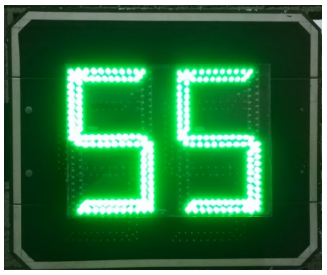
\includegraphics{figuras/cronometro.PNG}
    \end{center}
    \caption[Sistema de cronômetro]{Cronômetro marcador de tempo semafórico.}
    \label{cronometro}
\end{figure}

A placa de controle de contagem de tempo semafórico tem como finalidade realizar a contagem, e mostrar no \textit{display}, como mostrado na Figura \ref{cronometro}, do tempo de passagem veicular, enquanto o grupo focal estiver aceso no estado verde.

O microcontrolador utilizado é um AVR AT89S8253, que possui 40 pinos e capacidade de processamento de 8 \textit{bits}. Um cristal é utilizado, para gerar um \textit{clock} de 12 MHz, e cada instrução é realizada a cada 12 ciclos do \textit{clock}. O dispositivo é utilizado para realizar as funções de detectar o acendimento do verde no semáforo, contar, e salvar em memória, o tempo de verde e exibir o tempo em um \textit{display} de 7 segmentos.

O equipamento de contagem é instalado acoplado ao foco semafórico e é eletricamente conectado em paralelo com a fase verde do semáforo. Como não existe comunicação entre a placa de cronômetro e o controlador semafórico, o início da contagem do tempo é determinado pela detecção de acendimento do semáforo. Ao detectar a presença da rede elétrica, o microcontrolador busca na memória o valor da contagem de tempo de verde e inicia a contagem regressiva. Caso não exista valor salvo na memória, é carregado um valor padrão.

\begin{figure}[ht]
    \begin{center}
    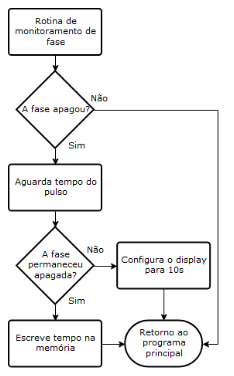
\includegraphics{figuras/fluxo_cron2.PNG}
    \end{center}
    \caption[Fluxograma do monitoramento do cronômetro]{Fluxo da rotina de monitoramento da fase veicular.}
    \label{fluxo_cron2}
\end{figure}

Após iniciar a contagem, o microcontrolador passa a monitorar a fase acesa, de acordo com a rotina demonstrada na Figura \ref{fluxo_cron2}. O controlador semafórico possui um método para indicar que o tempo de verde está próximo do fim, na forma de um pulso, com duração de 100 ms, durante o qual a alimentação é retirada da placa de contagem. Esse método é importante para assegurar o funcionamento correto do sistema nas determinadas situações:

\begin{itemize}
\item No ciclo inicial, em que o microcontrolador ainda não possui valor de tempo gravado na memória.
\item Após mudanças dos planos, quando o tempo de acendimento passar a ser diferente do tempo armazenado na memória.
\end{itemize}

O pulso é necessário nessas situações, pois são cenários em que ocorre dessincronização entre a placa de contagem e o controlador semafórico, e os \textit{displays} não exibem o tempo correto. Ao reconhecer o pulso, porém, a placa entra em sincronia com o controlador e exibe o valor correto no mostrador (o pulso indica que faltam 10 s de tempo de verde). Ao apagar o foco verde, o microcontrolador reconhece a ausência de alimentação por mais de 100 ms, e salva na memória o tempo do ciclo de acendimento.
No equipamento são utilizados dois \textit{timers} distintos para gerar interrupções. O primeiro é utilizado para a contagem do tempo e atualização da variável que é exibida nos displays. O segundo é utilizado para a contagem dos 100 ms para reconhecimento do pulso do controlador.

A placa de monitoramento de demanda de atuadores externos tem como finalidade acumular as demandas vindas de atuadores externos, ativados por pedestres para realizar a travessia de vias. A placa recebe um sinal, referente às atuações, do equipamento que realiza o registro das demandas, à medida que vão ocorrendo, e utiliza esse sinal para realizar cálculos referentes à quantidade e volume de demandas registradas.

Assim como a placa de controle de acendimento semafórico, o microcontrolador utilizado nessa placa é um PIC16F77, utilizando, também, um cristal de 20 MHz para gerar o \textit{clock}. As funções necessárias para essa placa são:

\begin{itemize}
\item Comunicação com a \ac{CPU}
\item Registro de atividades de atuadores externos
\item Cálculo de quantidade de demanda em um determinado intervalo de tempo
\item Cálculo de volume de demandas em um determinado intervalo de tempo
\end{itemize}

Para realizar a comunicação com a \ac{CPU}, é utilizada a porta serial do PIC, através de uma comunicação assíncrona. 
O circuito de monitoramento das demandas possui um optoacoplador, que é ativado quando o equipamento que registra as demandas envia o sinal por meio do pino externo, e o PIC detecta a atuação. Além desses dados, o PIC incrementa uma contagem cada vez que uma demanda é registrada, desse modo armazenando a contagem de atuação para cada detector.

Além da contagem de atuação, outra funcionalidade da placa é o armazenamento do volume das atuações. Para isso, o \textit{timer} do microcontrolador é utilizado. Durante a rotina de interrupção do \textit{timer}, o PIC identifica as demandas recebidas e calcula, durante uma janela de tempo (determinada pela \ac{CPU}), durante que porcentagem desse período as demandas ficaram ativas. Essas informações armazenadas são enviadas para a \ac{CPU}, por meio da porta serial, quando requisitadas.

\section{Placa de registro de demanda de pedestre}

A placa de registro de demanda de pedestre é um sistema de botoeira que registra as demandas realizadas pelo pedestre e envia um sinal para o controlador semafórico como aviso de ativação. O equipamento possui um botão, que deve ser pressionado para que ocorra o registro da demanda. 

O microcontrolador utilizado na placa é um PIC12F675, que possui 8 pinos e capacidade de processamento de 8 \textit{bits}. É utilizado o oscilador interno do PIC, com velocidade de \textit{clock} de 4 MHz, e cada instrução é realizada a cada 4 ciclos do \textit{clock}. Esse dispositivo é utilizado para detectar o pressionamento do botão que realiza a requisição de demanda, enviar um sinal ao controlador para identificar o registro, detectar o acendimento da fase de pedestres e ativar o funcionamento de um buzzer para indicar a travessia, no modo sonoro. 

O PIC realiza a leitura do botão por meio de \textit{polling} do pino (leitura do estado do botão a cada ciclo do programa principal). O equipamento possui dois modos de funcionamento, dependendo do pressionamento do botão, sendo eles o modo sonoro, caso o pressionamento ocorra por mais de 3 segundos, e o modo silencioso, no caso de pressionamento por menos de 3 segundos. A reconhecer o pressionamento do botão, a botoeira envia um sinal para o controlador semafórico, para requisitar o acionamento do plano de pedestres. 

Para ocorrer a ativação, um pino do PIC é utilizado para chavear um transistor \ac{TBJ}, que causa a ativação do relé, fazendo com que o sinal de 12 V seja enviado ao controlador ou ao \textit{buzzer}. 

Após a leitura do estado do botão e envio do sinal de demanda ao controlador, o equipamento realiza o monitoramento do semáforo de pedestres para determinar em qual estado se encontra.
No caso do modo de funcionamento sonoro, ao detectar o acendimento do foco verde, o equipamento ativa o funcionamento intermitente do \textit{buzzer}, na frequência de 1 Hz, para indicar ao pedestre que a travessia pode ser iniciada.

Ao detectar que o estado do semáforo passou de verde para vermelho intermitente, o equipamento ativa o funcionamento do \textit{buzzer}, dessa vez na frequência de 2 Hz, para indicar que o tempo de travessia se aproxima do fim. Ao identificar que o foco vermelho ficou aceso continuamente, o equipamento desliga o \textit{buzzer}.
Para controlar a frequência de ativação do \textit{buzzer}, é utilizada a interrupção de \textit{timer} do microcontrolador.

Durante o modo de funcionamento silencioso, a botoeira não realiza nenhuma ação, apenas monitora os acendimentos, sem ativar o \textit{buzzer}.

\section{Integração}
%Integração e aplicação (?)
%A aplicação do sistema é realizar o controle e monitoramento semafórico em vias urbanas, visando trazer organização e segurança ao trânsito. Estar de acordo com as normas técnicas vigentes (resoluções CET). 

Cada equipamento apresentado nesse trabalho desempenha um papel importante no controle e monitoramento da sinalização semafórica nas vias urbanas. Para que todos os processos ocorram de forma ordenada e sincronizada, é necessário que se realize a integração entre os sistemas com o controlador semafórico. 
%Essa integração pode ser dividida em duas etapas: o controle veicular e o controle de pedestres. Essas duas etapas 

\subsection{Controlador semafórico}

A integração dos sistemas se dá através do equipamento chamado controlador semafórico. O controlador semafórico é um sistema que tem como função a supervisão e o controle do trânsito, sendo composto por \textit{hardware} e \textit{software} capazes de prover uma rede semafórica inteligente e automatizada.

\begin{figure}[ht]
    \begin{center}
    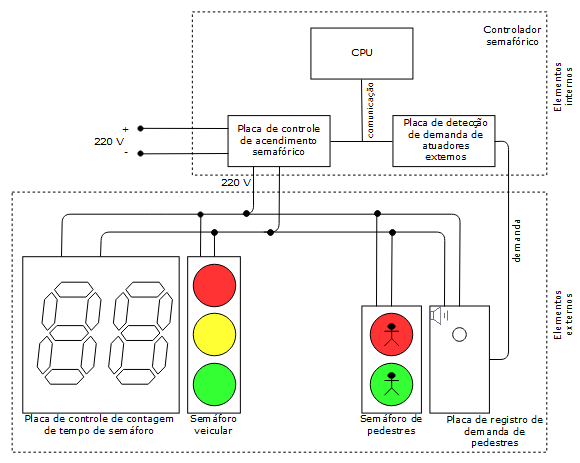
\includegraphics[width=0.7\textwidth]{figuras/diagrama_controlador.PNG}
    \end{center}
    \caption[Controlador semafórico]{Diagrama da integração do controlador semafórico.}
    \label{controlador}
\end{figure}

O controlador pode ser dividido em seus elementos internos e externos, que funcionam em conjunto para assegurar o correto funcionamento do sistema completo. A interação entre os elementos, que compoem o controlador, é mostrada na Figura \ref{controlador}. 

\subsubsection{Elementos internos}

Os elementos internos ao controlador são aqueles que se encontram fisicamente no gabinete do sistema. Esses elementos processam os dados medidos e recebidos dos elementos externos, e possuem comunicação com a \ac{CPU} do controlador.

A placa de controle de acendimento semafórico e a placa de detecção de demanda de atuadores externos são os dois elementos internos ao controlador e funcionam como interface entre a \ac{CPU} do controlador e os elementos externos, que não possuem comunicação.
A placa de controle de acendimento faz a conexão entre o controlador e os focos semafóricos (veicular e de pedestres) e a placa de contagem de tempo. A placa de detecção de demanda realiza a conexão entre o controlador e a placa de registro de demandas.

\subsubsection{Elementos externos}

Os elementos externos ao controlador são aqueles que não se encontram no gabinete do sistema. Esses elementos ficam à mostra e funcionam como interface entre o motorista e pedestre com o controlador semafórico. Não existem comunicação entre os elementos externos e a \ac{CPU} do controlador, portanto qualquer sinal necessário é transmitido aos elementos internos.

A placa de controle de contagem de tempo semafórico tem como finalidade indicar o tempo de acendimento restante no semáforo veicular, agindo como interface entre o usuário (motorista/pedestre) e os tempos calculados na \ac{CPU}. Já a placa de registro de demanda de pedestres possibilita a interação entre o pedestre e o controlador. Além dos dois sistemas, há ainda o foco semafórico como elemento externo ao controlador, funcionando em integração com a placa de controle de acendimento.

\subsection{Controle veicular}

O controle veicular é realizado pelas placa de controle de acendimento semafórico e placa de controle de contagem de tempo semafórico, assim como os focos semafóricos veiculares. A placa de acendimento é controlada pela \ac{CPU} do controlador semafórico, e é responsável pelo acendimento dos semáforos. A placa de contagem é instalada próxima ao foco semafórico.

Não há comunicação entre o foco semafórico, ou a placa de contagem, e a \ac{CPU} do controlador, pois a comunicação ocorre apenas entre a placa de acendimento e a \ac{CPU}. A única ligação entre os elementos são as linhas que levam tensão da rede elétrica da placa de acendimento até os outros dois equipamentos. A comunicação necessária se dá por essas linhas, sendo nesse caso o envio de um pulso de energia com o intuito de indicar a aproximação do fim do tempo de acendimento.

\subsection{Controle de pedestres}

O controle de pedestres é realizado pelas placa de detecção de demanda de atuadores externos e placa de registro de demanda de pedestres, assim como os focos semafóricos de pedestres. A placa de detecção é controlada pela \ac{CPU} do controlador semafórico, e é responsável por receber as demandas registradas pela placa de registro. A placa de de registro é instalada próxima ao ponto de travessia de pedestres.

Assim como no controle veicular, não há comunicação entre o foco semafórico de pedestres, ou a placa de registro de demandas, e a \ac{CPU} do controlador, apenas entre o controlador e a placa de detecção de demandas. As únicas ligações entre os elementos que realizam o controle de pedestres ocorrem entre o foco semafórico e a placa de registro (ligadas em paralelo na rede elétrica) e entre a placa de registro e a placa de detecção (linha de envio de demandas registradas). 